\documentclass[11pt]{article}
\usepackage[letterpaper,margin=.8in]{geometry}
% Shared font contract for manuscript text, math and figure labels.
% Matplotlib reads this preamble verbatim; do not use host-specific paths here.
\usepackage[T1]{fontenc}
\usepackage[utf8]{inputenc}
\usepackage{newtxtext,newtxmath}

\usepackage{graphicx,booktabs,array,amsmath,microtype,xurl}
\usepackage{placeins,caption}
\usepackage[numbers,sort&compress]{natbib}
\usepackage[hidelinks]{hyperref}
\usepackage{orcidlink}
\captionsetup{font=small,labelfont=normalfont,skip=5pt}
\setlength{\parskip}{.22em}
\setlength{\textfloatsep}{15pt plus 2pt minus 2pt}
\renewcommand{\topfraction}{.92}\renewcommand{\bottomfraction}{.88}\renewcommand{\textfraction}{.06}
\renewcommand{\floatpagefraction}{.8}
\makeatletter\setlength{\@fptop}{0pt}\let\tableinput\@@input\makeatother
\emergencystretch=2em\clubpenalty=10000\widowpenalty=10000
\graphicspath{{journal-figures/}}
\newcommand{\TotalObservations}{64,990}
\newcommand{\TotalLabelled}{63,685}
\newcommand{\TotalFrames}{29}
\newcommand{\PrimaryRuns}{351}
\newcommand{\TransferRuns}{45}
\newcommand{\NsclcDelta}{+0.097}
\newcommand{\NsclcLower}{+0.016}
\newcommand{\NsclcUpper}{+0.158}
\newcommand{\NsclcPca}{0.130}
\newcommand{\NsclcFull}{0.226}
\newcommand{\NsclcMean}{0.225}
\newcommand{\NsclcVsMean}{+0.002}
\newcommand{\NsclcVsMeanLower}{\ensuremath{-0.050}}
\newcommand{\NsclcVsMeanUpper}{+0.039}
\newcommand{\BccDelta}{\ensuremath{-0.026}}
\newcommand{\BccLower}{\ensuremath{-0.044}}
\newcommand{\BccUpper}{\ensuremath{-0.008}}
\newcommand{\BccPca}{0.168}
\newcommand{\BccFull}{0.141}
\newcommand{\BccMean}{0.149}
\newcommand{\BccVsMean}{\ensuremath{-0.008}}
\newcommand{\BccVsMeanLower}{\ensuremath{-0.037}}
\newcommand{\BccVsMeanUpper}{+0.028}
\newcommand{\BreastPca}{0.221}
\newcommand{\BreastFull}{0.154}
\newcommand{\BreastMean}{0.198}
\newcommand{\BreastNoContrast}{0.202}
\newcommand{\BreastDelta}{\ensuremath{-0.067}}
\newcommand{\TvaPca}{0.094}
\newcommand{\TvaFull}{0.149}
\newcommand{\TvaMean}{0.114}
\newcommand{\TvaNoContrast}{0.103}
\newcommand{\TvaDelta}{+0.056}
\newcommand{\HnsccPca}{0.271}
\newcommand{\HnsccFull}{0.219}
\newcommand{\HnsccMean}{0.211}
\newcommand{\HnsccNoContrast}{0.233}
\newcommand{\HnsccDelta}{\ensuremath{-0.052}}
\newcommand{\MibiPca}{0.210}
\newcommand{\MibiFull}{0.185}
\newcommand{\MibiMean}{0.149}
\newcommand{\MibiNoContrast}{0.209}
\newcommand{\MibiDelta}{\ensuremath{-0.025}}
\newcommand{\PositiveObjects}{5}
\newcommand{\NegativeObjects}{8}
\newcommand{\ContrastHelpsObjects}{5}
\newcommand{\ContrastHurtsObjects}{8}
\newcommand{\RegionTransferPcaAcc}{0.303}
\newcommand{\RegionTransferPcaBalanced}{0.257}
\newcommand{\RegionTransferSelfAcc}{0.336}
\newcommand{\RegionTransferSelfBalanced}{0.258}
\newcommand{\RegionTransferFullAcc}{0.382}
\newcommand{\RegionTransferFullBalanced}{0.312}
\newcommand{\CellTransferPcaAcc}{0.417}
\newcommand{\CellTransferPcaBalanced}{0.331}
\newcommand{\CellTransferSelfAcc}{0.400}
\newcommand{\CellTransferSelfBalanced}{0.326}
\newcommand{\CellTransferFullAcc}{0.339}
\newcommand{\CellTransferFullBalanced}{0.218}
\newcommand{\FullPeakMemory}{0.85}
\newcommand{\FullTimeMin}{0.78}
\newcommand{\FullTimeMax}{1.85}

\newcommand{\BccCommonKBetter}{2}
\newcommand{\BccCommonKDelta}{\ensuremath{-0.012}}
\newcommand{\BccNestedControlMean}{0.177}
\newcommand{\BccNestedDelta}{\ensuremath{-0.035}}
\newcommand{\BccNestedMax}{\ensuremath{-0.016}}
\newcommand{\BccNestedMin}{\ensuremath{-0.067}}
\newcommand{\BccNestedP}{0.125}
\newcommand{\BccNestedTesseraBetter}{0}
\newcommand{\BccVsPcaP}{0.125}
\newcommand{\BccVsPcaPositive}{0}
\newcommand{\BccWholeVsControlBetter}{0}
\newcommand{\BccWholeVsControlMean}{\ensuremath{-0.022}}
\newcommand{\BccWholeVsControlP}{0.125}
\newcommand{\BccWholeVsPcaMean}{\ensuremath{-0.025}}
\newcommand{\BccWholeVsPcaP}{0.125}
\newcommand{\BccWholeVsPcaPositive}{0}
\newcommand{\BelowSelfOnly}{8}
\newcommand{\CellTypeMean}{0.093}
\newcommand{\CellTypePca}{0.192}
\newcommand{\CellTypeTessera}{0.151}
\newcommand{\CellTypeTesseraLower}{4}
\newcommand{\GateAurocMax}{0.621}
\newcommand{\GateAurocMedian}{0.495}
\newcommand{\GateAurocMin}{0.385}
\newcommand{\GateBeaten}{12}
\newcommand{\GateExprAurocMedian}{0.536}
\newcommand{\GateObjects}{13}
\newcommand{\LungCommonKBetter}{5}
\newcommand{\LungCommonKDelta}{+0.166}
\newcommand{\LungGateLowMax}{81}
\newcommand{\LungGateLowMin}{50}
\newcommand{\LungGateMedianMax}{0.091}
\newcommand{\LungGateMedianMin}{0.011}
\newcommand{\LungNestedControlMean}{0.392}
\newcommand{\LungNestedDelta}{\ensuremath{-0.166}}
\newcommand{\LungNestedMax}{\ensuremath{-0.110}}
\newcommand{\LungNestedMin}{\ensuremath{-0.247}}
\newcommand{\LungNestedP}{0.0625}
\newcommand{\LungNestedTesseraBetter}{0}
\newcommand{\LungVsPcaP}{0.125}
\newcommand{\LungVsPcaPositive}{4}
\newcommand{\LungWeightTvdMax}{0.407}
\newcommand{\LungWeightTvdMin}{0.318}
\newcommand{\LungWholeVsControlBetter}{0}
\newcommand{\LungWholeVsControlMean}{\ensuremath{-0.147}}
\newcommand{\LungWholeVsControlP}{0.0625}
\newcommand{\LungWholeVsPcaMean}{+0.058}
\newcommand{\LungWholeVsPcaP}{0.188}
\newcommand{\LungWholeVsPcaPositive}{4}
\newcommand{\NoContrastSelfMaxGap}{0.004}
\newcommand{\NoGateAtLeast}{5}
\newcommand{\NoGateMean}{+0.019}
\newcommand{\PermNoContrastMaxGap}{0.004}
\newcommand{\StabilityPcaMin}{0.57}
\newcommand{\StabilityTesseraMax}{0.73}
\newcommand{\StabilityTesseraMin}{0.38}
\newcommand{\TransferCellFull}{0.218}
\newcommand{\TransferCellMeanSix}{0.096}
\newcommand{\TransferCellMeanTwoHundred}{0.072}
\newcommand{\TransferCellPca}{0.331}
\newcommand{\TransferCellTesseraBelowPca}{5}
\newcommand{\TransferRegionFull}{0.312}
\newcommand{\TransferRegionMeanSix}{0.297}
\newcommand{\TransferRegionMeanTwoHundred}{0.349}
\newcommand{\TransferRegionPca}{0.257}
\newcommand{\TransferRegionTesseraBelowPca}{0}
\newcommand{\WholeCellsMax}{100,335}
\newcommand{\WholeCellsMin}{21,368}

\newcommand{\BrCortexBestK}{200}
\newcommand{\BrCortexContig}{0.905}
\newcommand{\BrCortexGate}{0.457}
\newcommand{\BrCortexMean}{0.253}
\newcommand{\BrCortexNested}{0.286}
\newcommand{\BrCortexOracle}{0.341}
\newcommand{\BrCortexPca}{0.190}
\newcommand{\BrCortexTess}{0.416}
\newcommand{\BrCortexTessNested}{+0.131}
\newcommand{\BrCortexTessOracle}{+0.075}
\newcommand{\BrCortexTessPca}{+0.226}
\newcommand{\BrGateMax}{0.480}
\newcommand{\BrGateMin}{0.457}
\newcommand{\BrMerfishBestK}{100}
\newcommand{\BrMerfishContig}{0.931}
\newcommand{\BrMerfishGate}{0.468}
\newcommand{\BrMerfishMean}{0.175}
\newcommand{\BrMerfishNested}{0.425}
\newcommand{\BrMerfishOracle}{0.460}
\newcommand{\BrMerfishPca}{0.079}
\newcommand{\BrMerfishTess}{0.357}
\newcommand{\BrMerfishTessNested}{\ensuremath{-0.068}}
\newcommand{\BrMerfishTessOracle}{\ensuremath{-0.104}}
\newcommand{\BrMerfishTessPca}{+0.278}
\newcommand{\BrPcaGainMax}{0.342}
\newcommand{\BrPcaGainMin}{0.226}
\newcommand{\BrStarmapBestK}{30}
\newcommand{\BrStarmapContig}{0.921}
\newcommand{\BrStarmapGate}{0.480}
\newcommand{\BrStarmapMean}{0.491}
\newcommand{\BrStarmapNested}{0.568}
\newcommand{\BrStarmapOracle}{0.606}
\newcommand{\BrStarmapPca}{0.163}
\newcommand{\BrStarmapTess}{0.505}
\newcommand{\BrStarmapTessNested}{\ensuremath{-0.063}}
\newcommand{\BrStarmapTessOracle}{\ensuremath{-0.101}}
\newcommand{\BrStarmapTessPca}{+0.342}
\newcommand{\DevAllThirteenECoordMean}{+0.114}
\newcommand{\DevAllThirteenECoordNeg}{1}
\newcommand{\DevAllThirteenECoordP}{0.000488}
\newcommand{\DevAllThirteenECoordPos}{12}
\newcommand{\DevAllThirteenEMeanMean}{\ensuremath{-0.001}}
\newcommand{\DevAllThirteenEMeanNeg}{6}
\newcommand{\DevAllThirteenEMeanP}{0.835}
\newcommand{\DevAllThirteenEMeanPos}{7}
\newcommand{\DevAllThirteenEShufMean}{\ensuremath{-0.002}}
\newcommand{\DevAllThirteenEShufNeg}{7}
\newcommand{\DevAllThirteenEShufP}{0.664}
\newcommand{\DevAllThirteenEShufPos}{6}
\newcommand{\DevBccECoordMean}{+0.096}
\newcommand{\DevBccECoordNeg}{0}
\newcommand{\DevBccECoordP}{0.125}
\newcommand{\DevBccECoordPos}{4}
\newcommand{\DevBccEMeanMean}{\ensuremath{-0.006}}
\newcommand{\DevBccEMeanNeg}{3}
\newcommand{\DevBccEMeanP}{0.25}
\newcommand{\DevBccEMeanPos}{1}
\newcommand{\DevBccEShufMean}{\ensuremath{-0.009}}
\newcommand{\DevBccEShufNeg}{2}
\newcommand{\DevBccEShufP}{0.5}
\newcommand{\DevBccEShufPos}{2}
\newcommand{\DevLungECoordMean}{+0.100}
\newcommand{\DevLungECoordNeg}{1}
\newcommand{\DevLungECoordP}{0.125}
\newcommand{\DevLungECoordPos}{4}
\newcommand{\DevLungEMeanMean}{+0.001}
\newcommand{\DevLungEMeanNeg}{3}
\newcommand{\DevLungEMeanP}{0.938}
\newcommand{\DevLungEMeanPos}{2}
\newcommand{\DevLungEShufMean}{+0.002}
\newcommand{\DevLungEShufNeg}{3}
\newcommand{\DevLungEShufP}{0.875}
\newcommand{\DevLungEShufPos}{2}
\newcommand{\DevOthECoordMean}{+0.148}
\newcommand{\DevOthECoordNeg}{0}
\newcommand{\DevOthECoordP}{0.125}
\newcommand{\DevOthECoordPos}{4}
\newcommand{\DevOthEMeanMean}{+0.004}
\newcommand{\DevOthEMeanNeg}{0}
\newcommand{\DevOthEMeanP}{0.125}
\newcommand{\DevOthEMeanPos}{4}
\newcommand{\DevOthEShufMean}{+0.001}
\newcommand{\DevOthEShufNeg}{2}
\newcommand{\DevOthEShufP}{0.875}
\newcommand{\DevOthEShufPos}{2}
\newcommand{\HerAllECoordHi}{+0.261}
\newcommand{\HerAllECoordLo}{+0.120}
\newcommand{\HerAllECoordMean}{+0.194}
\newcommand{\HerAllECoordNeg}{0}
\newcommand{\HerAllECoordP}{0.00781}
\newcommand{\HerAllECoordPos}{8}
\newcommand{\HerAllENestedHi}{+0.053}
\newcommand{\HerAllENestedLo}{+0.004}
\newcommand{\HerAllENestedMean}{+0.027}
\newcommand{\HerAllENestedNeg}{2}
\newcommand{\HerAllENestedP}{0.0781}
\newcommand{\HerAllENestedPos}{6}
\newcommand{\HerAllEShufHi}{+0.015}
\newcommand{\HerAllEShufLo}{\ensuremath{-0.006}}
\newcommand{\HerAllEShufMean}{+0.005}
\newcommand{\HerAllEShufNeg}{2}
\newcommand{\HerAllEShufP}{0.469}
\newcommand{\HerAllEShufPos}{6}
\newcommand{\HerAllEUSixHi}{+0.011}
\newcommand{\HerAllEUSixLo}{\ensuremath{-0.005}}
\newcommand{\HerAllEUSixMean}{+0.003}
\newcommand{\HerAllEUSixNeg}{3}
\newcommand{\HerAllEUSixP}{0.438}
\newcommand{\HerAllEUSixPos}{5}
\newcommand{\HerAllTessNestedHi}{+0.002}
\newcommand{\HerAllTessNestedLo}{\ensuremath{-0.047}}
\newcommand{\HerAllTessNestedMean}{\ensuremath{-0.022}}
\newcommand{\HerAllTessNestedNeg}{6}
\newcommand{\HerAllTessNestedP}{0.141}
\newcommand{\HerAllTessNestedPos}{2}
\newcommand{\HerAllTessPcaHi}{+0.021}
\newcommand{\HerAllTessPcaLo}{\ensuremath{-0.053}}
\newcommand{\HerAllTessPcaMean}{\ensuremath{-0.015}}
\newcommand{\HerAllTessPcaNeg}{6}
\newcommand{\HerAllTessPcaP}{0.461}
\newcommand{\HerAllTessPcaPos}{2}
\newcommand{\HerAllTessUSixHi}{\ensuremath{-0.020}}
\newcommand{\HerAllTessUSixLo}{\ensuremath{-0.074}}
\newcommand{\HerAllTessUSixMean}{\ensuremath{-0.047}}
\newcommand{\HerAllTessUSixNeg}{7}
\newcommand{\HerAllTessUSixP}{0.0156}
\newcommand{\HerAllTessUSixPos}{1}
\newcommand{\HerAllUSixNestedHi}{+0.047}
\newcommand{\HerAllUSixNestedLo}{+0.004}
\newcommand{\HerAllUSixNestedMean}{+0.024}
\newcommand{\HerAllUSixNestedNeg}{2}
\newcommand{\HerAllUSixNestedP}{0.0781}
\newcommand{\HerAllUSixNestedPos}{6}
\newcommand{\HerBndECoordHi}{+0.456}
\newcommand{\HerBndECoordLo}{+0.157}
\newcommand{\HerBndECoordMean}{+0.309}
\newcommand{\HerBndECoordNeg}{0}
\newcommand{\HerBndECoordP}{0.00781}
\newcommand{\HerBndECoordPos}{8}
\newcommand{\HerBndENestedHi}{+0.074}
\newcommand{\HerBndENestedLo}{+0.009}
\newcommand{\HerBndENestedMean}{+0.042}
\newcommand{\HerBndENestedNeg}{1}
\newcommand{\HerBndENestedP}{0.0547}
\newcommand{\HerBndENestedPos}{7}
\newcommand{\HerBndEShufHi}{+0.016}
\newcommand{\HerBndEShufLo}{\ensuremath{-0.025}}
\newcommand{\HerBndEShufMean}{\ensuremath{-0.003}}
\newcommand{\HerBndEShufNeg}{4}
\newcommand{\HerBndEShufP}{0.805}
\newcommand{\HerBndEShufPos}{4}
\newcommand{\HerBndEUSixHi}{+0.005}
\newcommand{\HerBndEUSixLo}{\ensuremath{-0.029}}
\newcommand{\HerBndEUSixMean}{\ensuremath{-0.012}}
\newcommand{\HerBndEUSixNeg}{4}
\newcommand{\HerBndEUSixP}{0.258}
\newcommand{\HerBndEUSixPos}{4}
\newcommand{\HerBndGateAboveChance}{4}
\newcommand{\HerBndGateOverRaw}{4}
\newcommand{\HerBndSeamGate}{0.505}
\newcommand{\HerBndSeamGateHi}{0.544}
\newcommand{\HerBndSeamGateLo}{0.462}
\newcommand{\HerBndSeamPlain}{0.568}
\newcommand{\HerBndSeamPlainHi}{0.629}
\newcommand{\HerBndSeamPlainLo}{0.504}
\newcommand{\HerBndSeamRaw}{0.520}
\newcommand{\HerBndSeamRawGateHi}{+0.049}
\newcommand{\HerBndSeamRawGateLo}{\ensuremath{-0.017}}
\newcommand{\HerBndSeamRawGateMean}{+0.016}
\newcommand{\HerBndSeamRawGateNeg}{4}
\newcommand{\HerBndSeamRawGateP}{0.398}
\newcommand{\HerBndSeamRawGatePos}{4}
\newcommand{\HerBndSeamRawHi}{0.583}
\newcommand{\HerBndSeamRawLo}{0.453}
\newcommand{\HerBndSeamSmooth}{0.583}
\newcommand{\HerBndSeamSmoothGateHi}{+0.118}
\newcommand{\HerBndSeamSmoothGateLo}{+0.037}
\newcommand{\HerBndSeamSmoothGateMean}{+0.078}
\newcommand{\HerBndSeamSmoothGateNeg}{1}
\newcommand{\HerBndSeamSmoothGateP}{0.0156}
\newcommand{\HerBndSeamSmoothGatePos}{7}
\newcommand{\HerBndSeamSmoothHi}{0.650}
\newcommand{\HerBndSeamSmoothLo}{0.513}
\newcommand{\HerBndSeamSmoothPlainHi}{+0.023}
\newcommand{\HerBndSeamSmoothPlainLo}{+0.007}
\newcommand{\HerBndSeamSmoothPlainMean}{+0.015}
\newcommand{\HerBndSeamSmoothPlainNeg}{1}
\newcommand{\HerBndSeamSmoothPlainP}{0.0156}
\newcommand{\HerBndSeamSmoothPlainPos}{7}
\newcommand{\HerBndSeamSmoothRawHi}{+0.100}
\newcommand{\HerBndSeamSmoothRawLo}{+0.025}
\newcommand{\HerBndSeamSmoothRawMean}{+0.063}
\newcommand{\HerBndSeamSmoothRawNeg}{1}
\newcommand{\HerBndSeamSmoothRawP}{0.0234}
\newcommand{\HerBndSeamSmoothRawPos}{7}
\newcommand{\HerBndTessNestedHi}{+0.059}
\newcommand{\HerBndTessNestedLo}{\ensuremath{-0.080}}
\newcommand{\HerBndTessNestedMean}{\ensuremath{-0.008}}
\newcommand{\HerBndTessNestedNeg}{4}
\newcommand{\HerBndTessNestedP}{0.836}
\newcommand{\HerBndTessNestedPos}{4}
\newcommand{\HerBndTessPcaHi}{+0.068}
\newcommand{\HerBndTessPcaLo}{\ensuremath{-0.064}}
\newcommand{\HerBndTessPcaMean}{\ensuremath{-0.000}}
\newcommand{\HerBndTessPcaNeg}{5}
\newcommand{\HerBndTessPcaP}{1}
\newcommand{\HerBndTessPcaPos}{3}
\newcommand{\HerBndTessUSixHi}{\ensuremath{-0.000}}
\newcommand{\HerBndTessUSixLo}{\ensuremath{-0.132}}
\newcommand{\HerBndTessUSixMean}{\ensuremath{-0.062}}
\newcommand{\HerBndTessUSixNeg}{5}
\newcommand{\HerBndTessUSixP}{0.133}
\newcommand{\HerBndTessUSixPos}{3}
\newcommand{\HerBndThreeECoordHi}{+0.479}
\newcommand{\HerBndThreeECoordLo}{+0.160}
\newcommand{\HerBndThreeECoordMean}{+0.320}
\newcommand{\HerBndThreeECoordNeg}{0}
\newcommand{\HerBndThreeECoordP}{0.00781}
\newcommand{\HerBndThreeECoordPos}{8}
\newcommand{\HerBndThreeENestedHi}{+0.073}
\newcommand{\HerBndThreeENestedLo}{+0.009}
\newcommand{\HerBndThreeENestedMean}{+0.041}
\newcommand{\HerBndThreeENestedNeg}{1}
\newcommand{\HerBndThreeENestedP}{0.0547}
\newcommand{\HerBndThreeENestedPos}{7}
\newcommand{\HerBndThreeEShufHi}{+0.020}
\newcommand{\HerBndThreeEShufLo}{\ensuremath{-0.021}}
\newcommand{\HerBndThreeEShufMean}{+0.001}
\newcommand{\HerBndThreeEShufNeg}{2}
\newcommand{\HerBndThreeEShufP}{0.938}
\newcommand{\HerBndThreeEShufPos}{6}
\newcommand{\HerBndThreeEUSixHi}{+0.006}
\newcommand{\HerBndThreeEUSixLo}{\ensuremath{-0.023}}
\newcommand{\HerBndThreeEUSixMean}{\ensuremath{-0.008}}
\newcommand{\HerBndThreeEUSixNeg}{4}
\newcommand{\HerBndThreeEUSixP}{0.398}
\newcommand{\HerBndThreeEUSixPos}{4}
\newcommand{\HerBndThreeTessNestedHi}{+0.044}
\newcommand{\HerBndThreeTessNestedLo}{\ensuremath{-0.087}}
\newcommand{\HerBndThreeTessNestedMean}{\ensuremath{-0.020}}
\newcommand{\HerBndThreeTessNestedNeg}{5}
\newcommand{\HerBndThreeTessNestedP}{0.602}
\newcommand{\HerBndThreeTessNestedPos}{3}
\newcommand{\HerBndThreeTessPcaHi}{+0.033}
\newcommand{\HerBndThreeTessPcaLo}{\ensuremath{-0.066}}
\newcommand{\HerBndThreeTessPcaMean}{\ensuremath{-0.016}}
\newcommand{\HerBndThreeTessPcaNeg}{5}
\newcommand{\HerBndThreeTessPcaP}{0.57}
\newcommand{\HerBndThreeTessPcaPos}{3}
\newcommand{\HerBndThreeTessUSixHi}{\ensuremath{-0.005}}
\newcommand{\HerBndThreeTessUSixLo}{\ensuremath{-0.138}}
\newcommand{\HerBndThreeTessUSixMean}{\ensuremath{-0.069}}
\newcommand{\HerBndThreeTessUSixNeg}{5}
\newcommand{\HerBndThreeTessUSixP}{0.109}
\newcommand{\HerBndThreeTessUSixPos}{3}
\newcommand{\HerBndThreeUSixNestedHi}{+0.079}
\newcommand{\HerBndThreeUSixNestedLo}{+0.022}
\newcommand{\HerBndThreeUSixNestedMean}{+0.049}
\newcommand{\HerBndThreeUSixNestedNeg}{0}
\newcommand{\HerBndThreeUSixNestedP}{0.00781}
\newcommand{\HerBndThreeUSixNestedPos}{8}
\newcommand{\HerBndTwoECoordHi}{+0.485}
\newcommand{\HerBndTwoECoordLo}{+0.166}
\newcommand{\HerBndTwoECoordMean}{+0.327}
\newcommand{\HerBndTwoECoordNeg}{0}
\newcommand{\HerBndTwoECoordP}{0.00781}
\newcommand{\HerBndTwoECoordPos}{8}
\newcommand{\HerBndTwoENestedHi}{+0.088}
\newcommand{\HerBndTwoENestedLo}{+0.007}
\newcommand{\HerBndTwoENestedMean}{+0.044}
\newcommand{\HerBndTwoENestedNeg}{1}
\newcommand{\HerBndTwoENestedP}{0.0703}
\newcommand{\HerBndTwoENestedPos}{7}
\newcommand{\HerBndTwoEShufHi}{+0.020}
\newcommand{\HerBndTwoEShufLo}{\ensuremath{-0.024}}
\newcommand{\HerBndTwoEShufMean}{\ensuremath{-0.001}}
\newcommand{\HerBndTwoEShufNeg}{4}
\newcommand{\HerBndTwoEShufP}{0.914}
\newcommand{\HerBndTwoEShufPos}{4}
\newcommand{\HerBndTwoEUSixHi}{+0.003}
\newcommand{\HerBndTwoEUSixLo}{\ensuremath{-0.030}}
\newcommand{\HerBndTwoEUSixMean}{\ensuremath{-0.014}}
\newcommand{\HerBndTwoEUSixNeg}{4}
\newcommand{\HerBndTwoEUSixP}{0.188}
\newcommand{\HerBndTwoEUSixPos}{3}
\newcommand{\HerBndTwoTessNestedHi}{+0.057}
\newcommand{\HerBndTwoTessNestedLo}{\ensuremath{-0.094}}
\newcommand{\HerBndTwoTessNestedMean}{\ensuremath{-0.015}}
\newcommand{\HerBndTwoTessNestedNeg}{4}
\newcommand{\HerBndTwoTessNestedP}{0.719}
\newcommand{\HerBndTwoTessNestedPos}{4}
\newcommand{\HerBndTwoTessPcaHi}{+0.068}
\newcommand{\HerBndTwoTessPcaLo}{\ensuremath{-0.079}}
\newcommand{\HerBndTwoTessPcaMean}{\ensuremath{-0.003}}
\newcommand{\HerBndTwoTessPcaNeg}{5}
\newcommand{\HerBndTwoTessPcaP}{0.93}
\newcommand{\HerBndTwoTessPcaPos}{3}
\newcommand{\HerBndTwoTessUSixHi}{+0.005}
\newcommand{\HerBndTwoTessUSixLo}{\ensuremath{-0.171}}
\newcommand{\HerBndTwoTessUSixMean}{\ensuremath{-0.073}}
\newcommand{\HerBndTwoTessUSixNeg}{5}
\newcommand{\HerBndTwoTessUSixP}{0.172}
\newcommand{\HerBndTwoTessUSixPos}{3}
\newcommand{\HerBndTwoUSixNestedHi}{+0.100}
\newcommand{\HerBndTwoUSixNestedLo}{+0.022}
\newcommand{\HerBndTwoUSixNestedMean}{+0.058}
\newcommand{\HerBndTwoUSixNestedNeg}{0}
\newcommand{\HerBndTwoUSixNestedP}{0.00781}
\newcommand{\HerBndTwoUSixNestedPos}{8}
\newcommand{\HerBndUSixNestedHi}{+0.088}
\newcommand{\HerBndUSixNestedLo}{+0.023}
\newcommand{\HerBndUSixNestedMean}{+0.053}
\newcommand{\HerBndUSixNestedNeg}{0}
\newcommand{\HerBndUSixNestedP}{0.00781}
\newcommand{\HerBndUSixNestedPos}{8}
\newcommand{\HerClassesMax}{7}
\newcommand{\HerClassesMin}{4}
\newcommand{\HerCompECoordHi}{+0.304}
\newcommand{\HerCompECoordLo}{+0.125}
\newcommand{\HerCompECoordMean}{+0.216}
\newcommand{\HerCompECoordNeg}{0}
\newcommand{\HerCompECoordP}{0.00781}
\newcommand{\HerCompECoordPos}{8}
\newcommand{\HerCompENestedHi}{+0.039}
\newcommand{\HerCompENestedLo}{\ensuremath{-0.023}}
\newcommand{\HerCompENestedMean}{+0.012}
\newcommand{\HerCompENestedNeg}{2}
\newcommand{\HerCompENestedP}{0.523}
\newcommand{\HerCompENestedPos}{6}
\newcommand{\HerCompEShufHi}{+0.016}
\newcommand{\HerCompEShufLo}{\ensuremath{-0.007}}
\newcommand{\HerCompEShufMean}{+0.005}
\newcommand{\HerCompEShufNeg}{2}
\newcommand{\HerCompEShufP}{0.438}
\newcommand{\HerCompEShufPos}{6}
\newcommand{\HerCompEUSixHi}{+0.014}
\newcommand{\HerCompEUSixLo}{\ensuremath{-0.008}}
\newcommand{\HerCompEUSixMean}{+0.004}
\newcommand{\HerCompEUSixNeg}{2}
\newcommand{\HerCompEUSixP}{0.508}
\newcommand{\HerCompEUSixPos}{6}
\newcommand{\HerCompGateAboveChance}{7}
\newcommand{\HerCompGateOverRaw}{3}
\newcommand{\HerCompSeamGate}{0.522}
\newcommand{\HerCompSeamGateHi}{0.552}
\newcommand{\HerCompSeamGateLo}{0.479}
\newcommand{\HerCompSeamPlain}{0.566}
\newcommand{\HerCompSeamPlainHi}{0.615}
\newcommand{\HerCompSeamPlainLo}{0.506}
\newcommand{\HerCompSeamRaw}{0.550}
\newcommand{\HerCompSeamRawGateHi}{+0.067}
\newcommand{\HerCompSeamRawGateLo}{\ensuremath{-0.008}}
\newcommand{\HerCompSeamRawGateMean}{+0.029}
\newcommand{\HerCompSeamRawGateNeg}{3}
\newcommand{\HerCompSeamRawGateP}{0.227}
\newcommand{\HerCompSeamRawGatePos}{5}
\newcommand{\HerCompSeamRawHi}{0.609}
\newcommand{\HerCompSeamRawLo}{0.480}
\newcommand{\HerCompSeamSmooth}{0.580}
\newcommand{\HerCompSeamSmoothGateHi}{+0.091}
\newcommand{\HerCompSeamSmoothGateLo}{+0.025}
\newcommand{\HerCompSeamSmoothGateMean}{+0.058}
\newcommand{\HerCompSeamSmoothGateNeg}{1}
\newcommand{\HerCompSeamSmoothGateP}{0.0234}
\newcommand{\HerCompSeamSmoothGatePos}{7}
\newcommand{\HerCompSeamSmoothHi}{0.631}
\newcommand{\HerCompSeamSmoothLo}{0.517}
\newcommand{\HerCompSeamSmoothPlainHi}{+0.021}
\newcommand{\HerCompSeamSmoothPlainLo}{+0.008}
\newcommand{\HerCompSeamSmoothPlainMean}{+0.014}
\newcommand{\HerCompSeamSmoothPlainNeg}{0}
\newcommand{\HerCompSeamSmoothPlainP}{0.00781}
\newcommand{\HerCompSeamSmoothPlainPos}{8}
\newcommand{\HerCompSeamSmoothRawHi}{+0.046}
\newcommand{\HerCompSeamSmoothRawLo}{+0.008}
\newcommand{\HerCompSeamSmoothRawMean}{+0.030}
\newcommand{\HerCompSeamSmoothRawNeg}{1}
\newcommand{\HerCompSeamSmoothRawP}{0.0312}
\newcommand{\HerCompSeamSmoothRawPos}{7}
\newcommand{\HerCompTessNestedHi}{+0.042}
\newcommand{\HerCompTessNestedLo}{\ensuremath{-0.067}}
\newcommand{\HerCompTessNestedMean}{\ensuremath{-0.020}}
\newcommand{\HerCompTessNestedNeg}{5}
\newcommand{\HerCompTessNestedP}{0.562}
\newcommand{\HerCompTessNestedPos}{3}
\newcommand{\HerCompTessPcaHi}{+0.032}
\newcommand{\HerCompTessPcaLo}{\ensuremath{-0.064}}
\newcommand{\HerCompTessPcaMean}{\ensuremath{-0.019}}
\newcommand{\HerCompTessPcaNeg}{5}
\newcommand{\HerCompTessPcaP}{0.516}
\newcommand{\HerCompTessPcaPos}{3}
\newcommand{\HerCompTessUSixHi}{+0.033}
\newcommand{\HerCompTessUSixLo}{\ensuremath{-0.075}}
\newcommand{\HerCompTessUSixMean}{\ensuremath{-0.028}}
\newcommand{\HerCompTessUSixNeg}{6}
\newcommand{\HerCompTessUSixP}{0.367}
\newcommand{\HerCompTessUSixPos}{2}
\newcommand{\HerCompUSixNestedHi}{+0.043}
\newcommand{\HerCompUSixNestedLo}{\ensuremath{-0.032}}
\newcommand{\HerCompUSixNestedMean}{+0.008}
\newcommand{\HerCompUSixNestedNeg}{2}
\newcommand{\HerCompUSixNestedP}{0.711}
\newcommand{\HerCompUSixNestedPos}{6}
\newcommand{\HerGOther}{84.2}
\newcommand{\HerGOwn}{100.0}
\newcommand{\HerHOneVerdict}{was not met}
\newcommand{\HerHTwoVerdict}{was not met}
\newcommand{\HerPatients}{8}
\newcommand{\HerSpotsMax}{691}
\newcommand{\HerSpotsMin}{176}
\newcommand{\LandAnatKMax}{200}
\newcommand{\LandAnatKMin}{30}
\newcommand{\LandAnatN}{3}
\newcommand{\LandAnatOraclePos}{1}
\newcommand{\LandAnatSameMean}{+0.120}
\newcommand{\LandAnatSamePos}{3}
\newcommand{\LandCellKMax}{50}
\newcommand{\LandCellKMin}{6}
\newcommand{\LandCellN}{8}
\newcommand{\LandCellOraclePos}{1}
\newcommand{\LandCellSameMean}{+0.001}
\newcommand{\LandCellSamePos}{4}
\newcommand{\LandComputedKMax}{200}
\newcommand{\LandComputedKMin}{50}
\newcommand{\LandComputedN}{5}
\newcommand{\LandComputedOraclePos}{0}
\newcommand{\LandComputedSameMean}{+0.002}
\newcommand{\LandComputedSamePos}{4}
\newcommand{\LandGateAbove}{11}
\newcommand{\LandGateMax}{0.621}
\newcommand{\LandGateMedian}{0.497}
\newcommand{\LandN}{24}
\newcommand{\LandPathKMax}{200}
\newcommand{\LandPathKMin}{6}
\newcommand{\LandPathN}{8}
\newcommand{\LandPathOraclePos}{0}
\newcommand{\LandPathSameMean}{\ensuremath{-0.047}}
\newcommand{\LandPathSamePos}{1}
\newcommand{\LandRawOverGate}{19}
\newcommand{\LandTessOraclePos}{2}
\newcommand{\LandTessPcaPos}{10}
\newcommand{\LandTessSamePos}{12}
\newcommand{\RepAllMaxRange}{0.018}
\newcommand{\RepMaxRange}{0.052}
\newcommand{\RepMedianRange}{0.002}
\newcommand{\RepPairs}{24}
\newcommand{\RepSignChangesControl}{1}
\newcommand{\RepSignChangesSame}{0}

\newcommand{\CrcPatients}{3}
\newcommand{\CrcTissueSpots}{1934}
\newcommand{\CrcLabeledSpots}{1931}
\newcommand{\CrcQcExcluded}{173}
\newcommand{\CrcQcSpots}{1758}
\newcommand{\CrcTessMeanNeg}{3}
\newcommand{\CrcRawTessMeanNeg}{3}
\newcommand{\CrcTessMeanDelta}{\ensuremath{-0.026}}
\newcommand{\CrcTessMeanLow}{\ensuremath{-0.037}}
\newcommand{\CrcTessMeanHigh}{\ensuremath{-0.017}}
\newcommand{\CrcGate}{0.567}
\newcommand{\CrcGateLow}{0.507}
\newcommand{\CrcGateHigh}{0.648}
\newcommand{\CrcRaw}{0.573}
\newcommand{\CrcGateRawDelta}{\ensuremath{-0.006}}
\newcommand{\CrcGateRawLow}{\ensuremath{-0.029}}
\newcommand{\CrcGateRawHigh}{+0.008}
\newcommand{\CrcNoGateDelta}{+0.002}
\newcommand{\CrcNoGateLow}{\ensuremath{-0.001}}
\newcommand{\CrcNoGateHigh}{+0.005}
\newcommand{\CrcFitSeconds}{220}

\newcommand{\panelref}[2]{Fig.~\ref{#1}(#2)}
\newcommand{\suppanelref}[2]{Supplementary Fig.~#1(#2)}
\hypersetup{pdftitle={Neighborhood averaging accounts for spatial gains of Tessera in tumor spatial omics},pdfauthor={Zeyu Fu},pdfsubject={Matched and tuned spatial controls, component ablations and patient-held-out transfer}}
\title{Neighborhood averaging accounts for spatial gains of Tessera in tumor spatial omics}
\author{Zeyu~Fu$^{1,*}$\,\orcidlink{0009-0001-8329-0108}\\[3pt]
\small $^1$State Key Laboratory of Trauma and Chemical Poisoning,\\
\small Institute of Combined Injury, Chongqing Engineering Research Center for Nanomedicine,\\
\small College of Preventive Medicine, Army Medical University, Chongqing, China\\
\small $^*$Correspondence: \texttt{fuzeyu09@gmail.com}; \texttt{fuzeyu99@126.com}}
\date{}
\usepackage{float}
\usepackage[switch]{lineno}
\begin{document}\raggedbottom\maketitle
\modulolinenumbers[5]\linenumbers
\begin{abstract}
Spatial clustering models combine molecular measurements with tissue position, making it difficult to attribute improved agreement to learned components. We evaluated the released Tessera implementation using matched neighborhood averages, component removals and patient-held-out comparisons. In five lung patients, averages selected using the other patients exceeded Tessera's agreement with the supplied annotations. Removing learned gates did not consistently reduce agreement, whereas removing the neighbor-positive training term removed the gain. In an independently annotated breast cohort, a mean on the same graph exceeded Tessera for the complete annotation in seven of eight patients. The corresponding mean difference was nominally supported for that target, but compartment and tumor-boundary comparisons did not show the same inferential support. Transfer improved region classification while reducing cell-type classification, and a separate three-patient colorectal pilot did not establish an advantage over simple controls. These findings support neighborhood averaging and component ablations when interpreting this implementation. They do not establish a result for all graph encoders or replace comparisons with native implementations of other spatial methods.
\end{abstract}
\noindent\textbf{Keywords:} spatial transcriptomics; graph neural networks; spatial domains; baselines; ablation; patient-held-out evaluation.

\section{Introduction}
Spatial molecular profiling measures molecular state and position in the same tissue, and many methods now use position to cluster cells or capture spots into domains. A recurring question is whether a learned spatial encoder captures tissue organization that a simpler use of position would miss. We ask this question for one released graph encoder, Tessera, by asking how much of its agreement with supplied tissue annotations is explained by averaging each observation with its spatial neighbors at an appropriate scale.

The answer depends on what the annotation measures. Cell identity, neighborhood composition and tissue compartment are related but distinct targets: a molecular cell type can occur in several compartments, and a compartment can contain many cell types \citep{moses2022museum,rao2021architecture}. Spatial smoothing can therefore help recover a compartment while obscuring the cell types inside it. Tumor microenvironments make the distinction concrete because immune, stromal and epithelial populations intermix. Imaging-based panels, registered multi-assay breast measurements and serial-section Open-ST data each support several annotation types \citep{he2022cosmx,janesick2023breast,schott2024openst}. A region computed from neighboring cell types, a molecular category transferred from a reference and a boundary drawn by a pathologist answer different questions, so the origin of the annotation is part of the evaluation.

Spatial methods differ in graph construction, objective and assignment rule. STAGATE uses an adaptive graph-attention autoencoder, SEDR combines expression and spatial representations, GraphST applies graph self-supervised contrastive learning, and SpaGCN and SpaceFlow encode spatial consistency in other ways \citep{dong2022stagate,xu2024sedr,long2023graphst,hu2021spagcn,ren2022spaceflow}. Simpler approaches are competitive. SpatialPCA builds spatial correlation into dimension reduction, BANKSY augments each cell's features with a weighted neighborhood average, and MENDER summarizes multi-scale cellular context \citep{shang2022spatialpca,singhal2024banksy,yuan2024mender}. BANKSY in particular makes the balance between a cell and its neighborhood an explicit, tunable choice that spans cell typing and domain segmentation. Benchmarks compare many methods across technologies and tissues \citep{yuan2024benchmark,kang2025nar,chen2025imeta}, but a comparison of final partitions across methods conflates input processing, graph construction and clustering.

To attribute a gain to an encoder, the molecular input and assignment rule must be held fixed while the use of position is varied. Two further controls are needed. First, a simple spatial baseline must be given the same opportunity to choose its scale as the learned model has to fit its parameters; an untuned six-neighbor average is not that baseline. Second, the reference annotation's own construction must be considered. The lung regions used here were computed from cell-type frequencies among 200 spatial neighbors \citep{he2022cosmx,sun2026consensus}, so averaging at a similar scale is expected to recover them without any learned component.

The author-developed Tessera implementation evaluated here uses the released neural core with the field-aware graph and data adapters described below. Tessera combines learned edge gates, residual message passing, attention over network depths, feature reconstruction and a gate-weighted contrastive objective. Its gates were designed to down-weight edges that cross tissue boundaries. Each component makes a testable prediction: if the gates detect boundaries, they should separate annotation seams better than a trivial edge score and their removal should reduce agreement; if message passing captures structure beyond smoothing, Tessera should exceed a tuned neighbor average; and if the representation generalizes, it should help in patients that did not fit it. Coordinate identity and evaluation units also matter. Imaging fields can have separate local coordinate systems \citep{palla2022squidpy,yan2026alignment}, and thousands of cells from one field do not replace independent patients \citep{zimmerman2021pseudoreplication,roberts2017crossvalidation}.

We evaluated 13 assay objects: five NSCLC patients, four BCC patients, registered breast Visium, colorectal tubulovillous adenoma, an Open-ST lymph-node section and MIBI fields. Nine fixed arms, 29 spatial scale-control configurations per object plus PCA50, whole-section reruns, a corrected geometry null and patient-held-out transfer were scored with the same molecular input and assignment rule (\panelref{fig:workflow}{a--f}). We report every arm and seed, use patients as the unit of inference, and test each component prediction directly.

\begin{figure}[H]\centering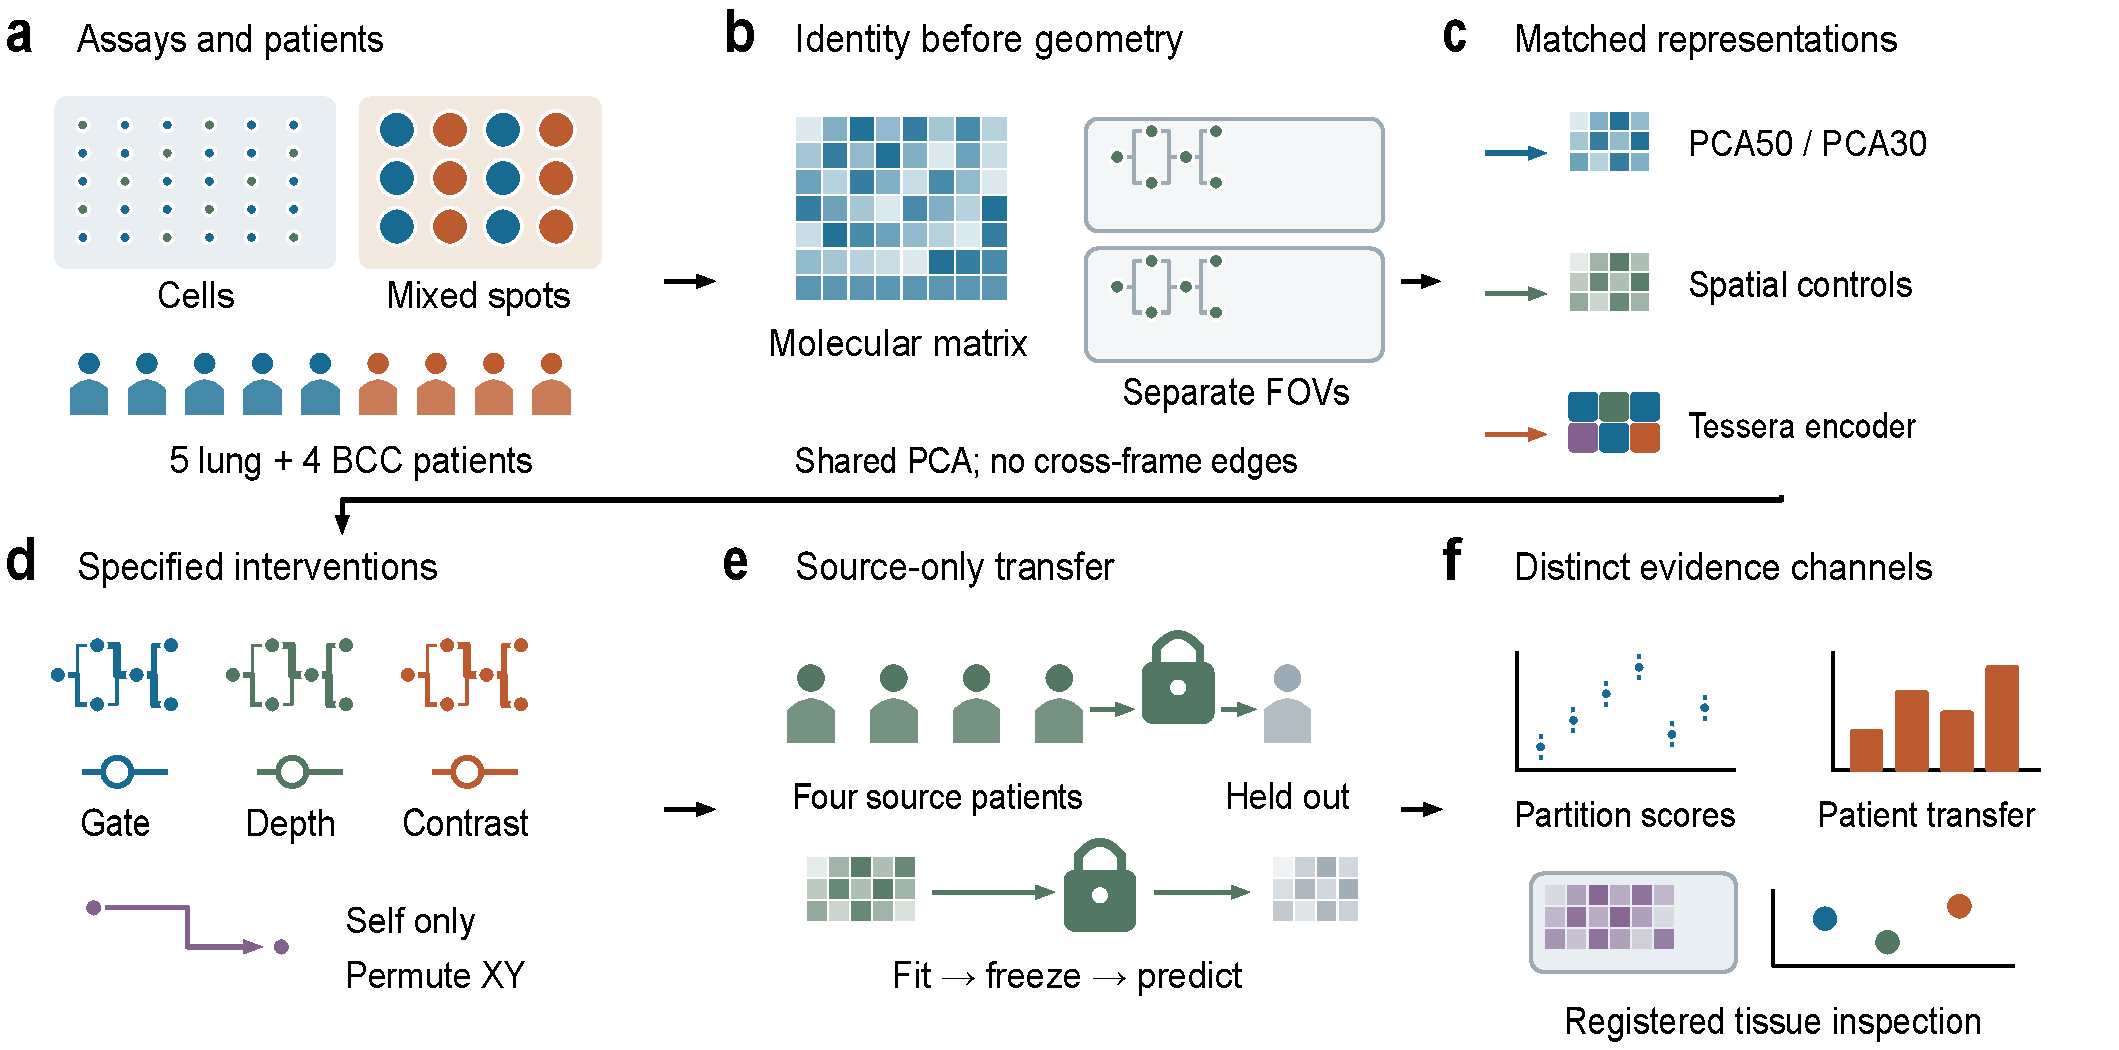
\includegraphics[width=\linewidth]{journal-figures/figure01-workflow.pdf}
\caption{Study design. (a) Assays and independent patients. (b) Molecular matrices and separate coordinate frames enter one common preprocessing. (c) Expression-only, simple spatial and learned representations form matched branches. (d) Component removals change one part of the encoder at a time. (e) In patient transfer, four source patients fit every transformation and weight before the fifth patient is mapped. (f) Partition, transfer and tissue-inspection readouts are reported separately. Icons are conceptual.}\label{fig:workflow}\end{figure}
\FloatBarrier

Two further sets of data test whether these conclusions travel. An independent cohort of eight HER2-positive breast tumors carries regions drawn by a pathologist on the stained tissue \citep{andersson2021her2st}, a construction that involves no averaging of neighboring expression, and three non-tumor tissues with anatomical labels \citep{maynard2021dlpfc,wang2018starmap,moffitt2018merfish} show whether the ordering depends on tissue. The independent-cohort all-label target and the comparison with patient-excluded tuned controls were fixed in writing before fitting. The untuned same-graph comparator, weighting controls, boundary variants and tissue panel were added after the initial results and are exploratory.



\section{Results}
\subsection{Matched averaging accounts for the principal lung comparison}
The comparison used the same molecular inputs and clustering rule for Tessera and its controls. In all five lung patients, an unweighted neighborhood average selected on the other patients exceeded Tessera's agreement with the supplied region annotation (\panelref{fig:comparison}{a,b}). Whole-section sensitivities and alternative clustering resolutions retained differences between targets and controls (\panelref{fig:comparison}{c,d}). The gain relative to expression-only coordinates therefore did not, on its own, identify an advantage of the learned encoder over matched spatial averaging.

\begin{figure}[H]\centering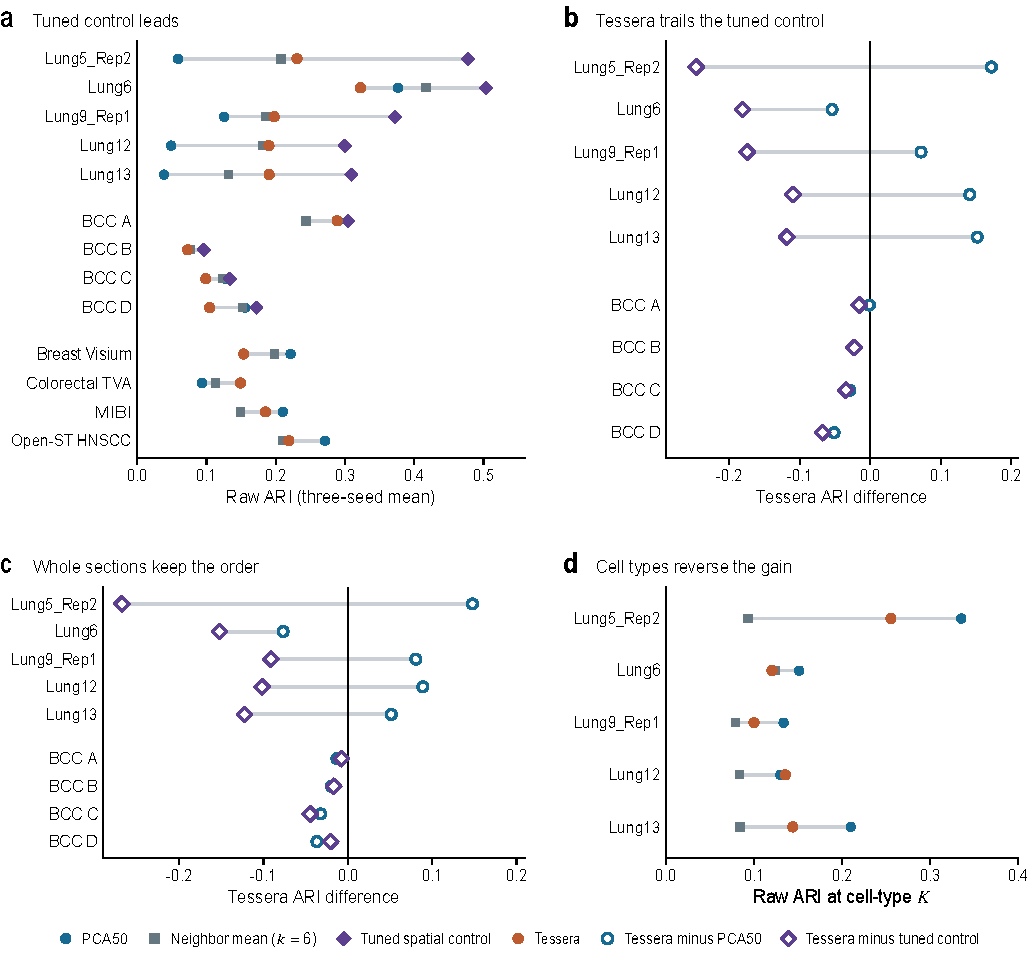
\includegraphics{journal-figures/figure03-comparison.pdf}
\caption{Tessera against expression-only, simple and tuned spatial controls. (a) Three-seed mean ARI per object; tuned controls are selected on other lung or BCC patients. (b) Bounded-field patient contrasts: Tessera minus PCA50 (open circles) and the nested control (open diamonds). (c) Uncapped whole-section sensitivity contrasts against PCA50 and fixed cohort-modal controls informed by the bounded analyses of the same patients. (d) Lung embeddings re-clustered at the cell-type cluster number and scored against supplied cell types.}\label{fig:comparison}\end{figure}
\FloatBarrier

\subsection{The contrastive term contributes more than the learned gates}
Removing learned gates did not consistently reduce lung agreement, whereas removing the neighbor-positive training term removed the principal gain (\panelref{fig:ablations}{a}). Gate discrimination of supplied seams was weaker than the plain feature difference in the relevant comparisons, and within-region and between-region gate distributions overlapped (\panelref{fig:ablations}{b,c}). Against the self-only encoder, Tessera improved agreement in four of five lung patients; Lung6 was the exception (\panelref{fig:ablations}{d}). These are component-specific results for the evaluated implementation, not a claim that spatial information or edge weights are universally useless.

\begin{figure}[H]\centering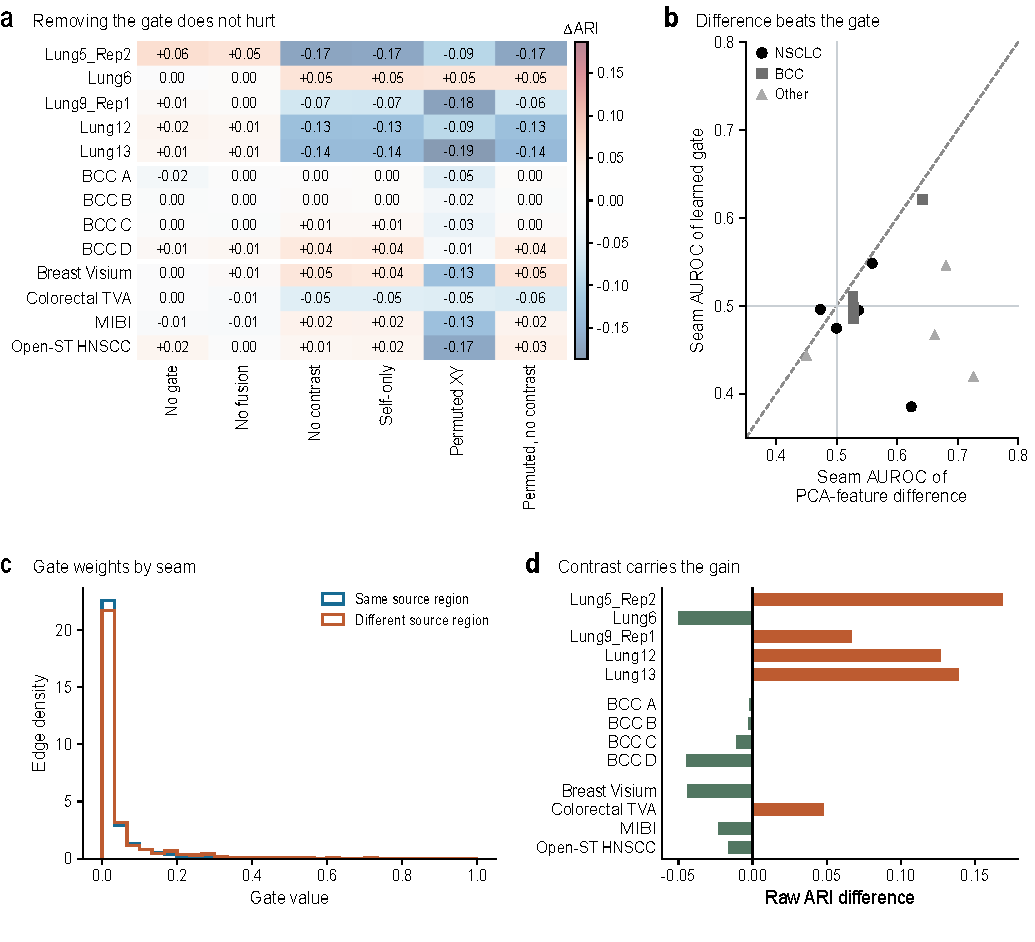
\includegraphics{journal-figures/figure04-ablations.pdf}
\caption{Which components carry the spatial effect. (a) Three-seed mean ARI of each control minus full Tessera; red favors the control. ``Permuted, no contrast'' trains on within-frame permuted coordinates without the contrastive term. (b) Seam discrimination by the last-layer gate versus by the plain PCA-feature difference on the same edges; points below the diagonal mean the gate is the weaker seam detector. (c) Last-layer gate distributions on edges within and across supplied regions in Lung5\_Rep2, seed 1. (d) Full Tessera minus the self-only encoder, the reference for the effect of measured geometry.}\label{fig:ablations}\end{figure}
\FloatBarrier

The lung maps and complete clustering-resolution and seed analyses are retained in the supplement. Three optimization seeds provide computational sensitivity within a patient. They do not add patients, and PCA seed differences reflect K-means initialization rather than independently fitted molecular representations.

\subsection{Patient transfer trades region accuracy for cell-type accuracy}
Each lung transfer fold fitted on four source patients and evaluated the excluded fifth patient. Tessera improved region balanced accuracy but reduced cell-type balanced accuracy in all five folds (\panelref{fig:transfer}{a,b}); ordinary accuracy gives the complementary summaries (\panelref{fig:transfer}{c,d}). A representation can therefore help one supplied annotation while harming another. The fixed neighborhood controls are descriptive, and their larger neighborhood setting was informed by the earlier lung analyses rather than selected independently within each fold.

\begin{figure}[H]\centering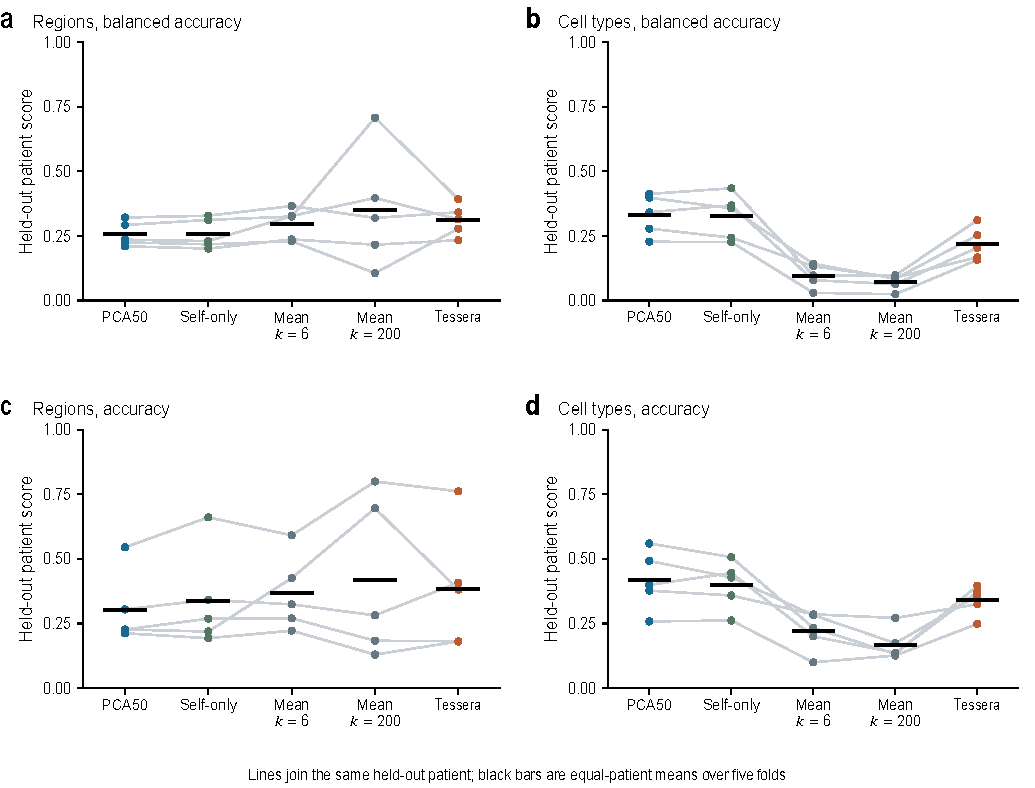
\includegraphics{journal-figures/figure10-patient-transfer.pdf}
\caption{Five patient-held-out NSCLC folds. (a, b) Region and cell-type balanced accuracy. (c, d) Accuracy. Four source patients fit scaling, PCA and the encoder; frozen parameters and source-category centroids map the held-out patient. Points are three-seed means for neural arms; fixed neighbor means (\(k=6,200\)) are deterministic descriptive controls, with \(k=200\) informed by earlier lung analyses, not fold-nested tuning. Lines join the same held-out patient; black bars are equal-patient means.}\label{fig:transfer}\end{figure}
\FloatBarrier

\subsection{The independent breast cohort supports a target-dependent result}
In eight independently annotated breast patients, the mean on Tessera's graph exceeded Tessera for the complete annotation in \HerAllTessUSixNeg{} patients, with mean Tessera-minus-control adjusted Rand index \HerAllTessUSixMean{} (\panelref{fig:external}{a}). Its descriptive sign-flip probability was \HerAllTessUSixP{}, with patient-bootstrap interval \HerAllTessUSixLo{} to \HerAllTessUSixHi{}. The same comparison was negative in \HerCompTessUSixNeg{} patients for named compartments and \HerBndTessUSixNeg{} for the tumor boundary, but the corresponding probabilities were \HerCompTessUSixP{} and \HerBndTessUSixP{} (\panelref{fig:external}{b,c}). The nominal result for the complete annotation is therefore not shared inferential support across all targets, and these same-graph extensions remain exploratory.

\begin{figure}[H]\centering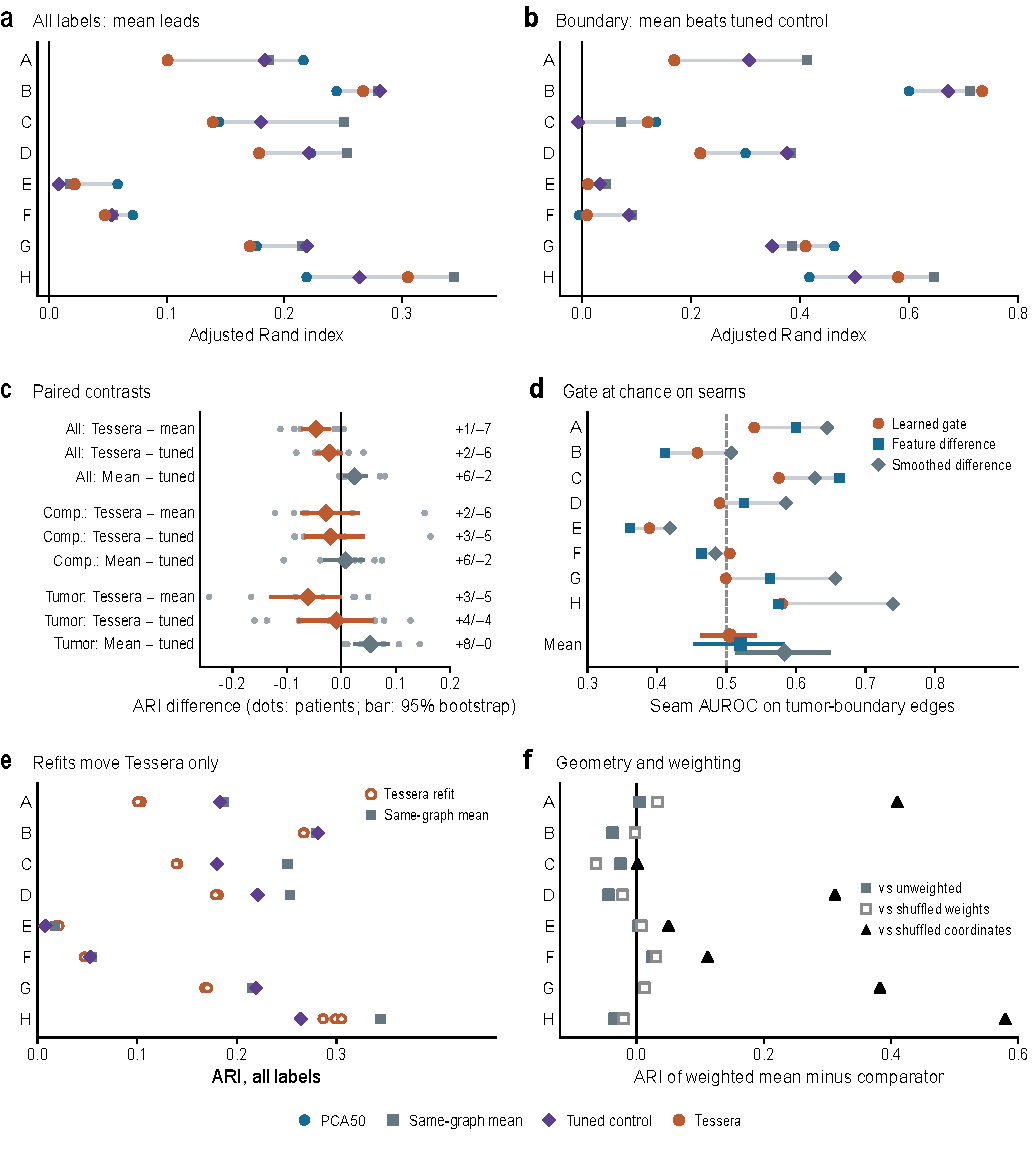
\includegraphics{journal-figures/figure15-external-cohort.pdf}
\caption{Independent pathologist-labelled cohort of eight HER2-positive breast tumors; rows A--H are patients. (a, b) Three-seed mean adjusted Rand index for all labels and for the tumor boundary: PCA50, the unweighted mean of neighbors on Tessera's graph, a tuned control selected on the other seven patients, and Tessera. (c) Paired differences for all labels (All), named compartments (Comp.) and the tumor boundary (Tumor); gray dots are patients, diamonds are means with 95\% bootstrap intervals, and the numbers count patients above and below zero. (d) Seam AUROC on tumor-boundary edges for the learned gate, the plain feature difference and the smoothed feature difference; the bottom rows give means with 95\% bootstrap intervals and the dashed line is chance. (e) Tessera's three replicate fits against the same-graph mean and the tuned control, all labels. (f) ARI of the weighted mean minus the unweighted mean, a mean with shuffled weights and a mean with shuffled coordinates, tumor boundary.}\label{fig:external}\end{figure}
\FloatBarrier

The learned gate's tumor-boundary discrimination was near chance; smoothing the molecular feature difference supplied more seam information (\panelref{fig:external}{d}). Repeated fits changed some comparisons with the tuned control but did not reverse the ordering against the same-graph mean (\panelref{fig:external}{e}). Weighting that mean did not provide a consistent clustering advantage over the unweighted mean, shuffled weights and shuffled-coordinate controls (\panelref{fig:external}{f}). Strong seam discrimination and useful clustering gain are distinct readouts.

\subsection{Further tissues preserve limits on generalization}
Across the 24 displayed objects, agreement differences depended on the tissue, annotation and neighborhood scale (\panelref{fig:landscape}{a--c}). The test-label-selected control envelope is descriptive rather than a held-out method comparison, and the gate and plain-feature seam scores measure a different target from clustering agreement (\panelref{fig:landscape}{d}). The plots do not establish a universal architecture ordering.

\begin{figure}[H]\centering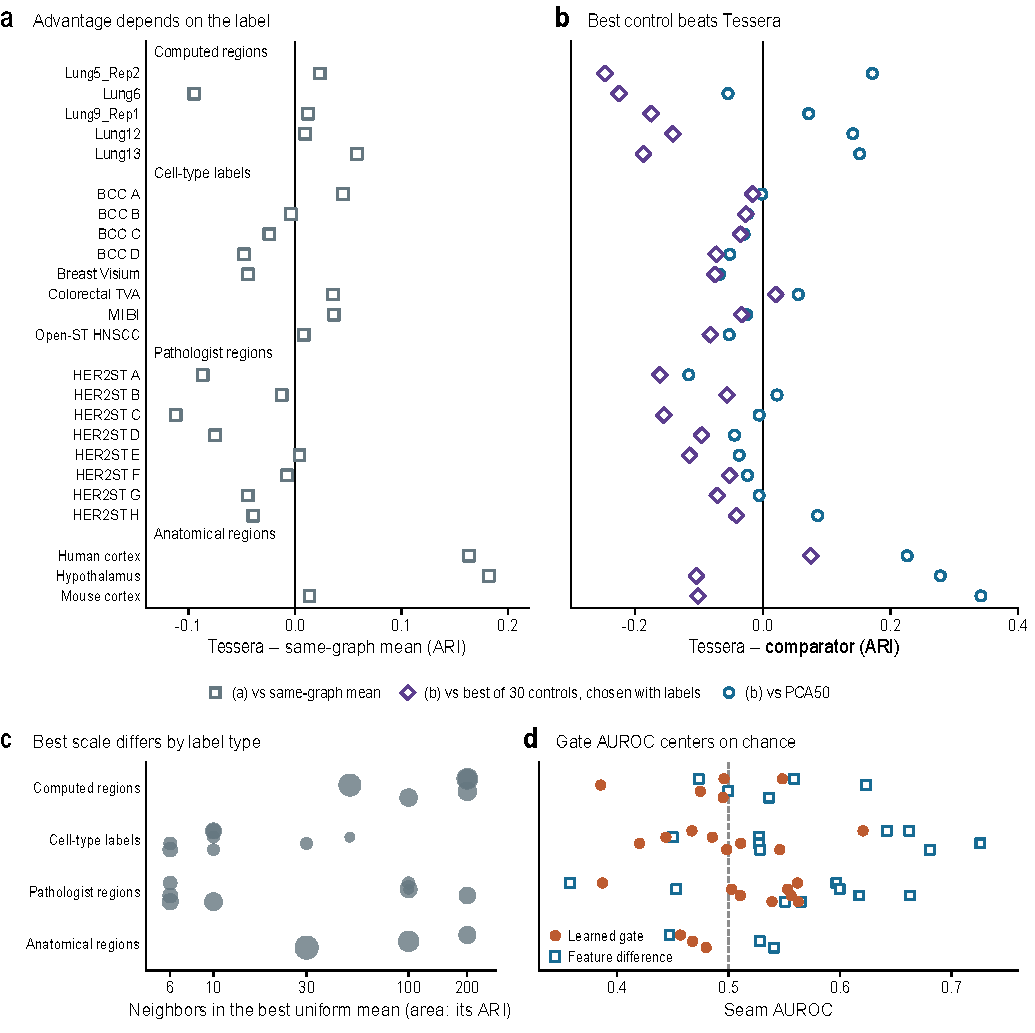
\includegraphics{journal-figures/figure17-tissue-landscape.pdf}
\caption{Twenty-four objects grouped by how the annotation was made: the 13 bounded objects, the eight independent patients and three further tissues. (a) Tessera minus the same-graph six-neighbor mean (ARI), which uses no label-based scale selection. (b) Tessera minus the best of 30 simple controls chosen with the test labels (diamonds) and minus PCA50 (circles). (c) Neighborhood size of the best uniform mean for each object; dot area is that mean's ARI. (d) Seam AUROC of the learned gate (filled) and the plain feature difference (open); the dashed line is chance.}\label{fig:landscape}\end{figure}
\FloatBarrier

In the separate three-patient colorectal pilot, the same-graph mean exceeded Tessera in all three patients, with mean difference \CrcTessMeanDelta{} and descriptive interval \CrcTessMeanLow{} to \CrcTessMeanHigh{}. Removing gates changed agreement by \CrcNoGateDelta{} on average, with interval \CrcNoGateLow{} to \CrcNoGateHigh{}. This interval does not demonstrate equivalence or a useful gating benefit. The gate had some above-chance seam information but did not demonstrate superiority to the plain feature difference. The pilot also did not establish advantage over raw features. Complete results are supplied in the Supplementary Results and pathology tables.

The study supports matched neighborhood averages and component removals when attributing Tessera's spatial gains. Native BANKSY and MENDER comparisons were not performed, some extension outputs do not support unrestricted fresh refitting, and small resource-selected cohorts limit population inference. These limits remain part of the conclusion.



























\section{Discussion}

Tessera's gains over expression-only clustering in lung tissue are real but are not evidence for its distinctive components. A neighbor mean whose scale was chosen on other patients outperformed it in every bounded lung input. Whole-section sensitivity analyses retained this ordering with a fixed 200-neighbor control informed by the same cohort; they test the sampling budget, not independent generalization. The lung regions were constructed from cell-type frequencies among 200 neighbors, and averaging at that scale recovers them without learning. An independent cohort whose regions a pathologist drew on the stained tissue, and which therefore was not built by neighborhood averaging, gave the same ordering: an untuned mean on Tessera's own graph exceeded the encoder in most patients, and so did a control tuned on the other patients. Spatial encoders should face neighborhood baselines with a comparable opportunity to choose their scale, and an unweighted same-graph mean, which needs neither labels nor tuning, is the cheapest informative comparator.

The component tests did not show a useful contribution from learned gating to lung agreement. The gates had small magnitudes, separated seams less well than a plain expression difference, and replacing them by uniform weights caused no systematic loss across these patients. Their relative weights were still heterogeneous after normalization, so small magnitude does not make the operator an unweighted mean. The ablation provides the mechanistic evidence: message passing with reconstruction alone reproduced the self-only encoder, while the neighbor-positive contrastive objective supplied the average lung gain. This finding concerns this released implementation, not gated graph networks in general; different gate objectives would need their own evaluation on untouched patients. In breast, gates gave near-chance tumor-seam AUROC; three anatomical tissues gave below-chance values, within the earlier 24-object median of \LandGateMedian{}. In colorectal tissue they carried weak seam information without demonstrated added value. Smoothing the feature difference over a neighborhood gave a better seam score, whereas reweighting a six-neighbor average by feature similarity showed no consistent advantage, so expression change at the seams carries information that neither the learned gate nor this simple reweighting turned into better domains at this resolution.

Target and clustering resolution both matter. At the primary cluster number, molecular or dominant-category targets favored expression-only clustering on BCC, breast, Open-ST and MIBI. Reducing the cluster number made BCC mixed, so that negative ordering is not universal. Within lung, the same embeddings that gained on regions lost on cell types, and transfer reproduced this trade-off with a different assignment rule. The 200-neighbor transfer control was informed by within-object analyses and is descriptive, although its transforms remain source-only. BANKSY explicitly weights the cell and its neighborhood \citep{singhal2024banksy}; our lightly weighted BANKSY-style control, not a native BANKSY run, was best in the bounded BCC selection. Multi-scale and composition representations address the region side of this trade-off \citep{yuan2024mender,liang2026cellniche}. Tessera's advantage was not uniform across annotations. It exceeded the same-graph mean in smooth anatomical tissue and in most computed lung regions but rarely in the pathologist-labelled patients, and it exceeded the best simple control chosen with the labels only in the cortex section used in its development and in colorectal TVA. Those exceptions show where a learned component could add structure beyond a neighborhood average, but one development section cannot establish it.

These results bear on how spatial methods are benchmarked. Comparisons with expression-only baselines reward any smoothing on spatially constructed targets, and untuned simple baselines understate what position alone can achieve. Benchmarks that already compare many native methods across platforms \citep{yuan2024benchmark,kang2025nar,chen2025imeta} would gain from including tuned and same-graph neighborhood averages and from reporting cell-type and domain targets separately. Seed variation also deserves attention: Tessera's partitions changed between seeds far more than PCA's, and repeated fits of identical code changed per-patient scores by up to \RepMaxRange{} ARI, so a single fitted partition is a weak basis for interpreting domain boundaries or for ranking methods whose scores differ by less than that.

Several limits apply. The study evaluates one released encoder at fixed hyperparameters; tuning it could change the findings, and fine-tuned or other spatial encoders were not tested. Five lung, four BCC and eight breast patients give coarse sign-flip summaries, and overlapping selection folds limit their inferential interpretation. The independent cohort has one pathologist, no second annotator and image registration that we inherited, and its weighting controls, boundary variants and tissue panel were chosen after the first comparison, so they are exploratory. The three non-tumor tissues are single sections that the encoder was benchmarked on earlier. Other annotations are computational or transferred labels, and the cluster number is label-informed. The Open-ST analysis remains a thinned subset, not a whole-section validation, and registered histology and protein channels support inspection only (Supplementary Fig.~S3). The three-patient colorectal pilot adds an untouched source, but cost selection, mixed labels and its disclosed QC sensitivity limit confirmation. Author H\&E overlays are not independent registration review. Stronger validation needs blinded adjudicated annotations and a patient sample designed for an effect margin. Calibration and selective abstention would require a separate protocol if uncertainty were claimed. A decisive test would use boundaries annotated independently by at least two readers in patients that informed neither method nor scale selection, together with a calibrated uncertainty readout.

In the tested lung and independent breast cohorts, simple neighborhood averaging accounts for much of the apparent gain over expression-only clustering. Component ablations identify the neighbor-positive contrastive objective as the source of the lung gain, while learned gates were dispensable there. Matched and tuned neighborhood averages should accompany architectural comparisons, with target construction, patient separation and computational variation reported explicitly.


\section{Methods}
\subsection{Implementation, data and matched comparisons}
We evaluated the released Tessera implementation, which constructs a spatial neighbor graph, weights edges with learned gates and fits a molecular representation with a neighbor-positive contrastive term. The primary panel contained 13 tumor-associated assay objects, including five independent lung patients. All compared methods used the same molecular inputs and clustering rule for an object. Shared preprocessing, annotation targets and patient identities are specified in the Supplementary Methods and input table.

Expression-only principal components and unweighted neighborhood means were the principal controls. Means were evaluated on Tessera's graph and across the recorded neighborhood-size grid. Tuned controls selected their setting using other patients; test-label-selected envelopes were displayed separately as descriptive bounds. Component removals tested learned gates, the contrastive term and other specified components. An edge gate was interpreted as an optimization weight, not an established tumor-boundary detector.

\subsection{Patient-level evaluation and external cohorts}
Clustering agreement used adjusted Rand index and normalized mutual information against each supplied annotation. Patient-paired contrasts retained all patients, and repeated optimization seeds quantified computational variability within a patient. Sign-flip probabilities and patient intervals were descriptive for the declared contrast; alternative targets and exploratory comparator extensions did not acquire confirmatory status from a nominal result. Five lung transfer folds fitted scaling, principal components and the encoder on the four source patients before mapping the held patient to source-category centroids.

An independently annotated breast cohort contained eight patients and separate complete-annotation, named-compartment and tumor-boundary targets. Same-graph weighting and boundary extensions were exploratory. Three further tissue sections and a separate three-patient colorectal pathology pilot tested additional contexts. The colorectal pilot did not establish advantage over raw features. Native BANKSY and MENDER implementations were not run, so the study does not provide a method-wide ranking of spatial approaches.

\subsection{Reproducibility and image provenance}
The Supplementary Methods preserve the encoder, graph, training, clustering, held-out selection, statistical and supplied-output procedures. Recorded saved outputs support the stated checks; a complete new fit of every extension is not claimed. Breast displays use author-generated coordinate maps and annotations. The colorectal images retain the source-specific attribution and open license documented in the image provenance record. No numeric result was changed by replacing the breast background or revising the document.

\subsection{Ethics and computational assistance}
The study reanalyzes measurements and annotations made public by the cited source studies. No new participants were recruited and no biological specimens were collected. Ethics approvals and consent arrangements for the original data collection are described in the source publications.

OpenAI Codex (OpenAI) assisted with code development, execution and checking of computational analyses, suggestions for analytical and methodological checks, manuscript drafting and restructuring, extensive language editing, and LaTeX and figure preparation. Reported numerical results were checked against saved outputs, and scripts and document builds were verified using the procedures described in this article and its Supplementary Information. AI-assisted critique and verification are preparation aids and do not constitute independent human peer review. The author directed the work and retains responsibility for the study design, data provenance, choice of analyses, scientific interpretation and final manuscript. No generative images were used as research data.





\section*{Data Availability}
No new biological measurements were collected. Data and annotations are available from the cited source studies under their original terms. The accompanying source package contains the evaluation code, written protocols, numerical result tables and editable manuscript and figure sources, including all reported independent-cohort replicate summaries. Large raw assays are acquired separately; included derived inputs, saved predictions and weights are enumerated in the manifest, and data-access instructions and the distinction between document reconstruction and full analysis reproduction are supplied with the package. The evaluated Tessera implementation is available at \url{https://github.com/PeterPonyu/tessera-st}, with an earlier public manuscript and implementation archive at DOI \url{https://doi.org/10.5281/zenodo.23101191}. That archive identifies the evaluated implementation; it does not archive the additional analyses reported here.


\section*{Code availability}
The analysis code, written protocols, numerical tables and supplied saved predictions are available at \url{https://github.com/PeterPonyu/tessera-st} and archived at software DOI \url{https://doi.org/10.5281/zenodo.23308077}. The archive defines which scores can be reconstructed from saved predictions and which require fresh fitting on separately acquired public assays. The earlier implementation archive remains the identifier of the evaluated release.
The software archive is the frozen computational evidence. The present submission revision and its editable document sources are separately versioned in the same repository.


\section*{Additional Information}
The author developed and maintains the Tessera implementation evaluated in this study. This developer role is disclosed as a relevant non-financial interest. The author declares no competing financial interests and no other competing interests. This research received no external funding.
{\small\setlength{\bibsep}{2pt}\bibliographystyle{naturemag}\bibliography{base_refs,new_refs}\par}

\section*{Author contributions}
Z.F. conceived the study, implemented the methods and evaluation, performed the analyses and wrote the manuscript.

\end{document}
